\cotefile{78}
\scanpage{2}
\margin{(\unsure{47v|47r})}
Polygônes réguliers

Chap I
% archive sheet number: 1

\scanpage{3}
\uline{Chap I}\qquad Introduction au Point de vue affine

\deleted{\uline{Point de vue affine}}

\textcircled{1} \uline{Définition \unsure{de|du} départ}

$E$ plan affine sur corps (disons \ldots) $k$. Un \uline{polygône}
\margin{\uline{Déf}}(déployé) dans $E$ est une partie finie \inserted{$S$} de $E$
(ensemble des sommets) \deleted{de cardinal $\geq 3$}, \uline{munie} d'une
``structure polygonale combinatoire'' i.e. d'une
partie à deux éléments $\omega=\{u,u^{-1}\}$ de $\unsure{\mathfrak{S}|\circlearrowright}_S$ qui soient
des permutations circulaires inverses l'une de l'autre (ce qui implique $n\geq3$). Les droites
joignant deux sommets contigus sont appelées les côtés\inserted{(en corr. 1-1 avec les côtés \unsure{comb})}\,; $\unsure{\omega|u}$ est \inserted{appelé} l'une des orientations de $P$. Si $n=\operatorname{card}S$,
c'est aussi le cardinal de l'ens des côtés -- on dit que $P$ est un $n$-polygône.

\margin{\unsure{pré-Déf|pre-Déf|re-Déf}}On dit que $P$ est \uline{régulier} si tout
autom combinatoire de \inserted{$Q=$} $(S,\omega)$ -- i.e. tout
élément du normalisateur \inserted{$G$} de $\omega$ dans $\mathfrak{S}_S$ --
se prolonge de façon unique en un autom
affine de $E$\,; il suffit bien sûr de l'exiger pour
\deleted{\unsure{les|des}} un système de gén, p.ex. \inserted{pr un $u\in\omega$} $u$ et une symétrie
$\sigma_s$ p.r. à un sommet $s$, ou une symétrie $\sigma_a$
p.r. à un \deleted{\unsure{côté}} \inserted{côté} $a$ [en fait, si $s$ et $a$ sont
incidents, deux \inserted{quelc} parmi les trois él. $\sigma_s,\sigma_a,u=\sigma_a\sigma_s$
forment \deleted{des} \inserted{un syst. de} générateurs]. Pour des raisons
techniques, on exige que les $u\in\omega$
(ou ce qui revient au $=$, les él. du
groupe \inserted{cyclique} $G^{\unsure{\bullet|0}}$ \unsure{engendré|engendrés} -- appelé \uline{groupe des
rotations} du polygône comb -- se réalisent
% archive sheet number: 2

\scanpage{4}
par des autom \uline{unimodulaires}, \deleted{\unsure{ils sont|il est}} On
comprendra mieux par la suite la nature
exacte de cette restriction (en étudiant
le pt de vue projectif)\,; disons pour
l'instant qu'on verra qu'il revient au
$=$ d'exiger $\sigma_a$ (l'un ou tous, \unsure{cel|cela}
revient au $=$ puisqu'ils sont conjugués)
est une réflexion -- i.e. laisse invariant
une droite. On verra aussi que cette
restriction est automatiquement satisfaite
\uline{sauf} dans le cas d'un polygône régulier
à $2p$ côtés en car $p$ ($p$ nb premier
impair) -- p.ex. l'hexagone en car. 3.

% slanted
\margin{\uline{Devrait remonter}}
NB \quad On fera attention que dans la définition
du polygône général, on avait défini
les côtés comme des \uline{droites} de $E$
-- on a une application \deleted{surjective} de
l'ens des côtés combinatoires \uline{sur} l'ens
des côtés géométriques. On dira
que le polygône est \uline{propre} si pour un sommet
$s\in S$ et un côté combinatoire $\{s',s''\}$, $s$
\figure{\begin{tikzpicture}[x=1cm,y=1cm]
\draw (0,0)--(.87,.28);
\end{tikzpicture}}
\figure{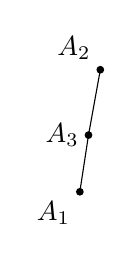
\begin{tikzpicture}[x=1cm,y=1cm]
\draw (.02,0)--(.13,.72)--(.28,1.55);
\fill (.02,0) circle (1.4pt) node[below left] {$A_1$};
\fill (.13,.72) circle (1.4pt) node[left] {$A_3$};
\fill (.28,1.55) circle (1.4pt) node[above left] {$A_2$};
\end{tikzpicture}}
\figure{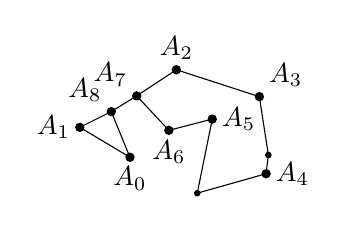
\begin{tikzpicture}[x=.95cm,y=.95cm]
\coordinate (a1) at (0,1.04); \coordinate (a8) at (.42,1.25);
\coordinate (a7) at (.76,1.46); \coordinate (a2) at (1.29,1.81);
\coordinate (a3) at (2.40,1.45); \coordinate (a4) at (2.49,.42);
\coordinate (a5) at (1.77,1.15); \coordinate (a6) at (1.19,1.00);
\coordinate (a0) at (.67,.64);
\draw (a0)--(a1)--(a8)--(a7)--(a2)--(a3)--(2.52,.67)--(a4)--(1.57,.16)--(a5)--(a6)--(a7);
\draw (a8)--(a0);
\foreach \p/\t/\d in {a0/0/below,a1/1/left,a2/2/above,a3/3/above right,a4/4/right,a5/5/right,a6/6/below,a7/7/above left,a8/8/above left}
{\fill (\p) circle (1.7pt) node[\d] {$A_{\t}$};}
\fill (1.57,.16) circle (1.2pt); \fill (2.52,.67) circle (1.2pt);
\end{tikzpicture}}
% archive sheet number: 3

\scanpage{5}
est incident au côté géométrique $D(s',s'')$
\uline{ssi} $s$ est incident au côté combinatoire, i.e.
$s=s'$ ou $s=s''$\,; ceci implique bien entendu
que les côtés géom corr. 1-1 aux côtés
combinatoires. On verra que les polygônes
réguliers (\unsure{même|mê} sans la condition unimodulaire)
sont \inserted{\unsure{néc|sic|aussi}} propres.

\figure{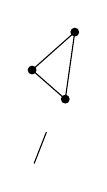
\begin{tikzpicture}[x=.86cm,y=.86cm]
\draw (0,.47)--(.63,1.03)--(.49,.04)--cycle;
\foreach \p in {(0,.47),(.63,1.03),(.49,.04)}{\fill \p circle (1.6pt);}
\draw (.21,-.45)--(.03,-.91);
\end{tikzpicture}}
La condition d'unicité dans la définition
du polygône régulier équivaut évidemment
à dire que $S$ engendre aff\textsuperscript{t} $E$, ou encore
que $S$ n'est pas \deleted{sur} \inserted{contenu dans} une droite. Il
revient au $=$ \deleted{que} de dire que
trois sommets consécutifs $s_0,s_1,s_2$ \uline{donnés}
sont non alignés [suffisance claire, pour la
nécessité on voit que si $d_0=D(s_0,s_1)$, on aurait
sinon \deleted{\unsure{$d$|$d_1$}} $d_0=u(d_0)$ [$us_0=s_1,\ldots$], donc
tous les $d_i$ égaux puisque $u$ transitif
sur l'ens des côtés, absurde \ldots].

% slanted
\margin{p\textsuperscript{t} de vue \unsure{voisin|inverse} fixer $\Pi$ (le ``schéma combinatoire'') \unsure{parler des|pour des|plutôt des} polygônes et \unsure{non après|ns après} \unsure{réguliers|s'agiter|épinglés}.}
Épinglage d'un polygône géom. par
un pol. comb $\Pi$ -- un polygône
géom. $\Pi$ épinglé\,: revient à la donnée
d'un couple \deleted{\unsure{$(S,\varphi)$|$(P$}} $(\Pi,\varphi)$, $\Pi=(S,\omega)$
polyg comb, $\varphi:S\longrightarrow E$ application injective
% archive sheet number: 4

\scanpage{6}
À vrai dire, l'\deleted{application}\inserted{injectivité} de l'application sur
les sommets, alors que l'application \deleted{\unsure{sur}} des
côtés comb vers les côtés géom peut
n'être pas injective, est \unsure{anachronique|encore que}
dans le cas non propre [\deleted{\unsure{en|on|où}} \deleted{dans le cas propre} la donnée
du polygône géom \inserted{propre} équivaut à la donnée
de l'ens des sommets et de l'ens
des côtés, satisfaisant les conditions suivantes\,: 
tt sommet incident à ex. deux côtés, tt
\unsure{côtés|côté} incident à exactement une \unsure{arête},
\deleted{\unsure{tout}} plus condition de connexité combinatoire\ldots]
La bonne notion est
donc celle de \uline{repr.} \inserted{(ou \uline{réalisation})} \uline{géom} d'un polyg.
combinatoire, qui revient à la donnée
de \uline{deux} applications -- sur l'ens des
sommets \uline{et} sur l'ens des droites --
respectant les relations d'incidence\ldots.
(Lorsque deux sommets incidents ont
\deleted{\unsure{l'image des pt de vue sommets}}
\deleted{\unsure{l'un des sommets a}} \inserted{\unsure{tjrs}} des images
\deleted{\unsure{pour être un polygône|pour être un polygone}} distinctes
par l'application $\varphi_{\mathrm{sommets}}$, cette dernière
suffit à elle seul à déterminer la réalisation,
et elle peut être choisie arbitrairement,
% archive sheet number: 5

\scanpage{7}
\uline{I bis}\qquad \uline{Exemples sur} $k=\mathbb{R}$

Prenons
\[
E=\mathbb{C} \tag*{(1)}
\]
regardé comme plan sur les réels. \deleted{\unsure{Soient}}Soit
\deleted{$\unsure{\zeta|z}$} $\zeta$ une racine \uline{primitive} \unsure{$n$:ième|$n$-ième} de 1 $\unsure{\big\}|:|,}$
\deleted{posons} (racine de 1 d'ordre $n$)
\[
\zeta^n=1,\qquad \zeta^d\ne 1\quad\text{si}\quad d\mid n,\deleted{\unsure{d|1}}1\leq d<n
\tag*{\deleted{\unsure{(a)|(2)}}(2)}
\]
posons
\[
s_i=\zeta^i\qquad i\in\mathbb{Z}/n\mathbb{Z}\tag*{(3)}
\]
avec la structure polygonale \inserted{combinatoire} standard.
\inserted{Les $s_i$ distincts car $\zeta$ racine \uline{primitive}.}
Soient $\sigma,u\in\deleted{\mathit{Aff}}\mathit{Gl}_{\mathbb{R}}(E)\subset\mathit{Aff}(E)$ définis par
\[
\left\{\begin{aligned}
\sigma z&=\bar z &&\unsure{\sigma|z}\in\\
uz&=\zeta z
\end{aligned}\right.
\tag*{\(\begin{aligned}&\text{(4)}\\&\deleted{\unsure{(5)}}\end{aligned}\)}
\]
donc on a
\[
\left\{\begin{aligned}
\sigma s_i&=s_{-i}\\
us_i&=s_{i+1}
\end{aligned}\right.\tag*{(5)}
\]
donc on a un $n$-polygone régulier, $P_{\zeta}$.

On vérifiera \deleted{que} aisément (et on retrouvera
ça dans un contexte plus général)
que
a) $P_\zeta$ isom \unsure{à|:} $P_{\zeta'}$ ssi $\zeta'=\zeta$ ou $\zeta'=\zeta^{-1}$
(ou encor, posant $\unsure{\alpha(\zeta)|\alpha()}=\zeta+\zeta^{-1}$, ssi $\alpha(\zeta)=\alpha(\zeta')$)

b) Tout polygône régulier \deleted{dans \illegible{1}}
un plan affine sur $\mathbb R$ est isom. à un $P_\zeta$.
% archive sheet number: 6

\scanpage{8}
Si $\unsure{\mathscr{T}|\mathcal{T}}$ est le groupe des racines de l'unité dans $\mathbb{C}$, \deleted{donc} i.e. le ss-gpe de
torsion de $\mathbb{C}^{\unsure{\times|*}}$, qui est isomorphe à
$\mathbb{Q}/\mathbb{Z}$, \deleted{donc dans $\mathscr{T}$ il y a un unique \unsure{élém|élément} d'ordre 2, savoir $-1$, engendre l'unique ss-gpe cyclique d'ordre 2, $\{\pm1\}\subset\mathscr{T}$}
donc $\pm1$ opère sur
$\mathscr{T}$ (écrit additivement pour les besoins de la
cause) et \deleted{$\unsure{\mathscr{T}/\pm1|\mathscr{T}/\{\pm1\}}$} l'ens des classes
d'isom de \unsure{polygones|polygônes} réguliers sur $\mathbb R$
est en corr. biunivoque canonique
avec $\bigl(\mathscr{T}/\{\pm1\}\mathbin{\backslash}\{0_{\mathscr{T}}\}\bigr)$ où $0_{\mathscr{T}}$ est l'image
dans le quotient $\mathscr{T}/\{\pm1\}$ de l'élt. nul de $\mathscr{T}$.

On a pour quatre pts consécutifs $s_i,s_{i+1},s_{i+2},s_{i+3}$
\[
(s_{i+3}-s_i)=\deleted{\unsure{\zeta|(+}}r(s_{i+2}-s_{i+1})
\]
\figure{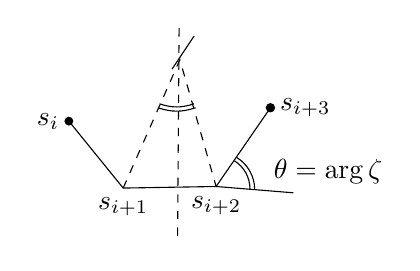
\begin{tikzpicture}[x=1cm,y=1cm]
\coordinate (s0) at (0,.91); \coordinate (s1) at (.69,.06);
\coordinate (s2) at (1.87,.08); \coordinate (s3) at (2.56,1.08);
\coordinate (t) at (1.41,1.69);
\draw (s0)--(s1)--(s2)--(s3); \draw (s2)--(2.85,0);
\draw[dashed] (s1)--(t)--(s2); \draw[dashed] (1.40,2.09)--(1.38,-.63);
\draw (1.31,1.57)--(1.59,1.99);
\draw (1.15,1.13) to[bend right=18] (1.59,1.13);
\draw (1.13,1.08) to[bend right=18] (1.61,1.08);
\draw (2.36,.04) arc[start angle=0,end angle=58,radius=.48];
\draw (2.30,.05) arc[start angle=0,end angle=58,radius=.42];
\fill (s0) circle (1.6pt) node[left] {$s_i$};
\node[below] at (s1) {$s_{i+1}$}; \node[below] at (s2) {$s_{i+2}$};
\fill (s3) circle (1.7pt) node[right] {$s_{i+3}$};
\node[right] at (2.48,.27) {$\theta=\arg\zeta$};
\end{tikzpicture}}
où $r$ est un nb \uline{réel} qui ne dépend
que de $\zeta$ (pas de $i$) en fait
\[
r=1+\underbrace{(\zeta+\zeta^{-1})}_{2\cos\arg\zeta}
\]
En effet,
\[
\frac{\zeta^{i+3}-\zeta^i}{\zeta^{i+2}-\zeta^{i+1}}\deleted{\unsure{=}}=
\frac{\zeta^3-1}{\zeta^2-\zeta}=
\frac{\zeta^2+\zeta+1}{\deleted{\unsure{\zeta^2-}}\zeta}=1+(\zeta+\zeta^{-1})
\]
% archive sheet number: 7

\scanpage{9}
Si on étend les scalaires du plan \inserted{vect} réel
\unsure{au|en} plan vectoriel complexe, l'hom \inserted{$u_{\zeta}$} de
multiplication complexe par $\zeta$ (pour tt nb
complexe) se décompose, suivant deux
droites ``isotropes'' canoniques en
la matrice \inserted{diagonale} $(\zeta,\zeta^{-1})$,
\diagram{\begin{tikzcd}[ampersand replacement=\&,row sep=small,column sep=small]
E\arrow[d,dash]\arrow[dr,shift right=2pt,"\varphi_1"']\arrow[dr,shift left=2pt,"\varphi_2"]\&{}\\
\mathbb{R}\arrow[r]\&\mathbb{C}
\end{tikzcd}}
\[
\left\{\begin{aligned}
\varphi_1(z)\deleted{\unsure{\mathbb C=\mathrm{id}_{\mathbb C}|z=\mathrm{id}_{\mathbb C}}}&=z\\
\varphi_2(z)&=\bar z
\end{aligned}\right.
\]
\[
E_{\mathbb C}\simeq\mathbb C^2
\]
le pt 1 de $E$ devient
le pt $s_0=(1,1)$ de $\mathbb C^2$,
et $s_i$ devient le pt de coordonnées
complexes $(\zeta^i,\zeta^{-i})=u_\zeta^i(s_0)$. La symétrie
p.r. au sommet $s_0$, i.e. $z\longrightarrow\bar z$, est
transformé en l'autom $(\deleted{\unsure{-|x}}x,y)\longmapsto(y,x)$
symétrie des deux axes. On verra que
cette structure du $n$-polygône régulier
est typique, pour les corps \inserted{alg clos} de car.
première à $n$\,; et pour ceux-ci on a la $=$
classification des $n$-polygônes réguliers \inserted{$((n,p)=1)$} que
celle indiquée dans le cas du corps des
réels. (NB Le fait que dans le cas
particulier $k=\mathbb R$, \uline{bien que $k$ ne soit pas
alg} clos, on ait la $=$ classification, est
remarquable et demande de l'attention\ldots
% archive sheet number: 8

\scanpage{10}
% The writing is upside down in the scan. The oblique cancelling strokes traverse the sheet.
\[
\deleted{u(\operatorname{Tr}v\,\mathrm{id}-v)=(\operatorname{Tr}v)u-uv}
\]
\[
\deleted{\operatorname{Tr}u\bar v=\operatorname{Tr}u\operatorname{Tr}v-\operatorname{Tr}(uv)}
\qquad \deleted{\unsure{2\operatorname{Tr}\dot v|2\operatorname{Tr}v}}
\]
\[
\deleted{\det u+\det v=}
\]
\[
\deleted{\det(u+v)=\det u+\det v+
(\underbrace{\operatorname{Tr}u\operatorname{Tr}v-\operatorname{Tr}uv}_{\varphi(u,v)})}
\]
\diagram{\begin{tikzcd}[ampersand replacement=\&,column sep=small,row sep=small]
\deleted{\cdot}\&\deleted{\widetilde X}\arrow[r,phantom,"\deleted{\unsure{\sim|/}}"]\&\deleted{\widetilde Y}\&\deleted{u}\\
\deleted{(}\&{}\&\deleted{\unsure{M|\mathcal M}}\&{}
\end{tikzcd}}
\[
\deleted{ux}\qquad\deleted{u\ \text{\uline{unimodulaire}}}
\]
\[
\deleted{\begin{pmatrix}\lambda&u\\0&\lambda'\end{pmatrix}}
\qquad\deleted{\left\{\begin{aligned}ux&=0\\\operatorname{Tr}u&=0\end{aligned}\right.}
\]
\deleted{$D$ comme \unsure{point} ou comme \unsure{fais\textsuperscript{t} gche|faisceau droit|point fixe} $\unsure{\mathscr L|\mathcal L}\subset\unsure{\mathscr{N}l(A)|\mathit{Nil}(A)}$ des $u$ tels que}
\[
\deleted{uD\subset D,\quad\operatorname{Tr}u=0}
\]
\[
\deleted{u\quad\begin{pmatrix}\lambda&u\\&-\lambda\end{pmatrix}}\qquad
\begin{aligned}&\deleted{\unsure{u}}\\&\deleted{E/D}\end{aligned}
\]
\[
\begin{aligned}
&\deleted{\unsure{u+|u}}\\
&\deleted{0\subset\underbrace{\mathcal O_S\subset\unsure{\widetilde V|\widetilde{\mathscr V}|\sqrt{\mathcal{J}}}}\subset\mathscr L}\qquad\deleted{\lambda}
\end{aligned}
\]
\[
\deleted{\begin{pmatrix}\lambda&\\0&\lambda\end{pmatrix}}\qquad
\deleted{X\longrightarrow\mathbb P(\widetilde V/\mathcal O_S)}
\]
\[
\deleted{\operatorname{Tr}u=}\quad \deleted{uD\subset D}
\]
\[
\deleted{u=\lambda+v}\qquad\deleted{u=\lambda\,\mathrm{id}+v}\qquad
\deleted{v\ \text{\unsure{nilp.t|nilpotent}}}
\]
\[
\deleted{\unsure{u}}\qquad\deleted{x}\qquad\deleted{\underline{\operatorname{Tr}u=0}}
\quad\deleted{\unsure{u^2=0}}\quad\deleted{\underline{\det u=0}}
\]
\[
\begin{aligned}&\deleted{\unsure{u|v}^{\unsure{2|n}}=0}\\&\deleted{\lambda\unsure{\cdot|{}^{2}}}\end{aligned}
\]
% archive sheet number: 9

\scanpage{11}
\textcircled{II}\quad\uline{Épinglages et repères}.

Un \uline{repère} d'un polygône combinatoire est
un couple $(s_0,d_0)$ d'un sommet et d'un côté incidents\,; il revient au $=$ de
se donner un couple $(s_0,s_1)$ de deux
sommets adjacents \deleted{\unsure{(ou encore|ou ce qui}} (prendre
$d_0=\{s_0,s_1\}$) ou d'un $s_0\in S$ et de $u\in\omega$
-- sommet et orientation -- (prendre $s_1=us_0$).

\uline{Prop} \uline{1} $\Gamma=\operatorname{Aut}(S,\omega)$ est \inserted{\unsure{simplemt|simplement}} transitif sur l'ens des repères -- \deleted{\unsure{qui est donc}} \inserted{i.e. celui-ci est} un torseur sous $\Gamma$.

C'est en. équivalent à ceci

\uline{Cor} 1 Soient $\Pi=(S,\omega)$, $\Pi'=(S',\omega')$ deux \deleted{\unsure{isom|isom.}} pol
comb \inserted{isomorphes}, et soit $r_0=(s_0,u)$ un repère de
$\Pi$. Alors l'application
\[
\begin{aligned}
\operatorname{Isom}(\Pi,\Pi')&\longrightarrow\operatorname{Rep}(\Pi')\\
\unsure{\theta|\Theta}&\longmapsto\theta(\unsure{r|r_0})
\end{aligned}
\]
est bijective. \unsure{$\vert$}

Un \uline{épinglage} d'un poly. comb. est
la donnée d'un repère (donc \uline{c'est} un
repère) -- \deleted{celui} \inserted{un épinglage (ou repère)} d'un polygône géom.
est un ép. du pol. comb sous-jacent.
Il revient au $=$ de \deleted{dire} se donner un $\Pi_0$-
% archive sheet number: 10

\scanpage{12}
épinglage, où $\Pi_0$ est le ``\unsure{$n$-polyg.|polyg.|$n$-poly.} combinatoire type''
% slanted
\margin{(i.e. \inserted{``le''} \deleted{\unsure{tout|deux}} \deleted{\unsure{le|l'un} \illegible{1} épinglé} pol. comb. épinglé -- i.e. muni d'un \uline{repère}\ldots)}
\uline{Cor. 2} Soient $P=(E,S,\omega)$, $P'=(E',S',\omega')$ deux
polygônes réguliers isomorphes, \deleted{Alors} le
premier étant épinglé \inserted{par un repère $r$}. Alors l'application
\[
\unsure{\Theta|\theta}\unsure{\longmapsto|\longrightarrow}\Theta(r)\,:\quad \operatorname{Isom}(P,P')\longrightarrow\operatorname{Rep}(E',S',\omega')
\]
est bijective.

\uline{Scholie} On peut dire encore\,: dans tte
classe d'isomorphie de $n$-polygônes
réguliers, les $n$-polygônes réguliers \uline{épinglés}
sont déterminés à \uline{isom} \uuline{unique} près.
[Idem bien sûr ds le cas purement
combinatoire]. \inserted{Bien sûr, les classes d'iso des uns et des autres se correspondent 1-1\ldots}

\uline{NB} Il y aura donc la question ``d'écrire''\
``\uline{le}'' espace affine $E$ dans lequel se
place $P$, en termes du type d'isomorphie
(i.e. de $n$ et d'un
``module'' $\alpha\in k$ convenable), \deleted{et l'angle
au sommet} et ceci fait, ``d'écrire''\
également \uline{les} \deleted{\unsure{côtés}} \inserted{sommets} $s_i$ ($0\leq i\unsure{\leq|<} n-1$).
% archive sheet number: 11

\scanpage{13}
\textcircled{III}\quad Polygônes $n$-réguliers et repr. du \uline{groupe} \inserted{diédral}

\deleted{\uline{Revenons au cas des polygônes réguliers}.}
\deleted{\unsure{S'il|Il|Soit} est $\Pi$ épinglé, \inserted{où $\Pi=(S,\omega=\{u,u^{-1}\})$,} et si \unsure{$\Gamma$ est le|$\Gamma$ est $k$}}
% slanted
\margin{\deleted{Question} Parler de l'épinglage (ou \uline{repère}) du pt de vue combinatoire (revient à la donnée, soit d'un couple $(s_0,d_0)$ d'un sommet et d'une \deleted{\unsure{arête}} \unsure{de|et}, soit au couple de deux sommets consécutifs $(s_0,s_1)$, soit au couple $(s_0,u)$ d'un sommet et d'une orientation. Donner la propriété de \uline{rigidification} (1)}
\[
\deleted{\Gamma=\operatorname{Aut}(\Pi)\qquad
\Gamma^{\unsure{\bullet|0}}=\text{ens des autom conservant l'orient.}}
\]
\deleted{on obtient une représentation}
\[
\deleted{\Gamma\xrightarrow{\varphi}\operatorname{Aut\,aff}(E)}
\]
\deleted{et $S$ \inserted{ensemble des sommets} est donc une orbite \unsure{ss|sous} $\Gamma$.}

\deleted{\unsure{du}} \inserted{Nous partirons du} \uline{pt de vue intrinsèque} \deleted{(non épinglé)}.

Le polygône $P=(S,\omega)$ détermine un
sous-groupe
\[
\Gamma\subset\operatorname{Aut\,aff}(E)
\]
isomorphe à un groupe diédral $D_n$
\[
\Gamma\simeq D_n\quad \inserted{n\in\mathbb N\ \text{convenable}}\quad
\text{(isomorphisme \uline{non} donné)}\tag*{(1)}
\]
et $S$ est une orbite de $\Gamma$ op. sur $E$
\[
S\in\deleted{\unsure{E/\Gamma|\Gamma}}\Gamma\backslash E\tag*{(2)}
\]
donc le ss-gpe $\Gamma$ étant donné, \deleted{$\unsure{E|S}$}
$S$ est déterminé quand on connaît
\uline{un} de ses sommets, soit
\[
\unsure{\cdot}\ s_0\in E\tag*{(4)}
\]
\deleted{\unsure{si que|à qu|À quelle}} Le polygône \unsure{$P$|$P_s$} est-il connu
par la connaissance de $(\Gamma,\deleted{s_0,}S)$,
i.e. la structure combinatoire \inserted{$\omega$} de $S$
résulte-t-elle de la connaissance du
ss-gpe $\Gamma\subset\deleted{\operatorname{Aut}}\unsure{\mathfrak S|\circlearrowright}_S$ de ses autom.?
% archive sheet number: 12

\scanpage{14}
\uuline{Non}, car ce groupe est le $=$ pour \deleted{la str}
$\omega=\{u,u^{-1}\}$ et $\omega^{(r)}=\{u^r,u^{-r}\}$ où $r\in\mathbb Z$, $(r,n)=1$.

Il faut donc en plus se donner une
partie
\[
\omega\subset\Gamma\tag*{(4)}
\]
avec
\[
\left\{\begin{aligned}
&\operatorname{card}(\omega)=2,\qquad\omega=\{u,u^{-1}\}\\
&\deleted{\unsure{\Gamma|\Gamma^0}}
\end{aligned}\right.\tag*{(5)}
\]
\deleted{\unsure{et|de}} telle que, si $\Gamma^{\unsure{0|\circ}}$ est le ss-gpe de $\Gamma$
engendré par $\omega$ (i.e. par \deleted{l'}un \uline{\unsure{seul|quelq.}} \deleted{\unsure{élémt}}
de ses éléments) on ait
\[
\left\{\begin{aligned}
&\operatorname{Card}\Gamma/\Gamma^0=2\\
&\Gamma/\Gamma^0\ \text{opère sur }\Gamma^0\ \text{par}\quad\lambda\longmapsto\lambda^{-1}\\
&\text{l'ext. }\Gamma\ \text{de }\Gamma/\Gamma^0\ \text{par }\Gamma^0\ \text{est semi-d.te,}\\
&\hspace{4em}\text{i.e. }\exists\,\sigma\in\Gamma,\ \sigma^2=1,\ \sigma\longmapsto\text{él\textsuperscript{t}}
\\&\hfill {-1}\ \text{de }\Gamma/\unsure{\Gamma_0|\Gamma_1|\Gamma^0}
\end{aligned}\right.\tag*{(6)}
\]
[\uline{NB} Ces conditions, qui précisent (1) \inserted{(modulo la condition que $\Gamma^0$ est fini)}
doivent bien sûr remplacer (2)]

En résumé, $P$ est déterminé
par la donnée

a) du ss-gpe $\Gamma\subset\mathit{Aff}(E)$

b) de la partie $\omega\subset\Gamma$
satisfaisant (5) (6)

c) de $S\in\Gamma\backslash E$ (ens des orbites)
% archive sheet number: 13

\scanpage{15}
Quelles conditions faut-il imposer à a) b) c)
pour que ces données proviennent d'un
polygône régulier? Signalons condition (6),
\figure{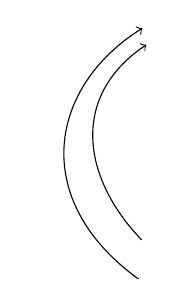
\begin{tikzpicture}[x=1cm,y=.7cm]
\draw[->] (.88,0).. controls (-.52,1.45) and (-.25,3.50)..(.93,4.55);
\draw[->] (.92,.71).. controls (.16,1.84) and (.01,3.32)..(.98,4.25);
\end{tikzpicture}}
% Both conditions are carried upward in the left margin; the written rows run (9), (8), (7).
\[
\inserted{\Gamma^{\unsure{0|\circ}}\ \text{fini}}\tag*{(7)}
\]
\[
\inserted{S\ \text{est un torseur sous }\Gamma^0}\tag*{(8)}
\]
et ensuite
\[
\deleted{\unsure{(7)|\text{et}}}\quad
\deleted{\unsure{\operatorname{card} S|\text{condition}}}\,
\left\{\begin{aligned}&S\ \text{n'est pas contenu ds une}\\&\text{droite de }E\end{aligned}\right.
\tag*{(9)}
\]
Ces \deleted{quatre} \deleted{\unsure{(6) à (9)}} conditions \inserted{(6 à 9)} suffisent, car la
structure de torseur sur $S$ sous $\Gamma^0$
met sur $S$ (grâce à $\omega\subset\Gamma^0$ \inserted{\unsure{et (7-)|et (7)}}) une
structure de $n$-polygone combinatoire
($n=\operatorname{card}\Gamma^0$) \inserted{-- on utilise (9) pour avoir $\Gamma\hookrightarrow\deleted{\operatorname{Aut}}\unsure{\mathfrak S|\circlearrowright}_S$ d'où $\omega\simeq\omega'\subset\mathfrak S_S$}\,;
\deleted{et si $\sigma\in\Gamma$ est comme ds (6), il induit un autom de $(S,\omega)$ qui renverse l'orientation, donc $\Gamma$ induit \unsure{et induit} \unsure{pas|pour} exactement le groupe des autom de}
$\Gamma'$ est son grpe des autom, on a évidemt
\diagram{\begin{tikzcd}[ampersand replacement=\&,column sep=small,row sep=0em]
\Gamma\arrow[r,hook,"\unsure{\sim|\omega}"]\&\Gamma'\\[-2pt]
\rotatebox{90}{$\subset$}\&\rotatebox{90}{$\subset$}\\[-2pt]
\Gamma^0\arrow[r,phantom,"\simeq"]\&\Gamma'{}^0
\end{tikzcd}}
qui induit un \uline{isom}orph.

Si on a \unsure{fixé|fixer|fixe} $n$, (7) devient.
\[
\operatorname{card}\Gamma^0\simeq\mathbb{Z}/n\mathbb{Z}.\tag*{$(7')$}
\]
% archive sheet number: 14

\scanpage{16}
On peut d'ailleurs remplacer la donnée c)
par la donnée
\[
S\in\unsure{\Gamma^0|\Gamma^\circ|\Gamma_0}\backslash E\tag*{c')}
\]
\margin{plus sympathique car on \unsure{passe au|tourne au|prend un|prend une} quotient par un groupe cyclique}
\deleted{\unsure{sont}} et les conditions à mettre sont alors (7) \inserted{et (9)}, puis
\[
\deleted{\Gamma^0\ \text{opère \uline{fid.} sur } S
\quad\left\{\begin{aligned}&\text{ou encor, si }s_0\in S\\&\text{et }u\in\omega\ \text{fixés}\\&us_0\ne s_0\end{aligned}\right.}
\tag*{\deleted{(8')}}
\]
\deleted{\unsure{ou, en av|ou, en ayant}}
\[
\deleted{\unsure{\Gamma|S}\quad\operatorname{card}S=\operatorname{card}(\Gamma^0)=n}\tag*{\deleted{$(8'')$}}
\]
% slanted
\margin{alors \deleted{\unsure{?}}, comme par (9), et $\Gamma\subset\mathit{Aff}(E)$, $\Gamma$ donc $\Gamma^0$ opère \uline{fidèlement} \deleted{dans} \inserted{sur} $S$ on en conclut \deleted{que} (comme $\Gamma^0$ est cyclique et transitif sur $S\ne\varnothing$) que $S$ est un torseur sous $\Gamma^{\unsure{\bullet|0}}$\ldots}
\unsure{puis} Il faut assurer que $S$ est
stable \deleted{sous} $\Gamma$ i.e. est une orbite sous
$\Gamma$, \deleted{Si on choisit \unsure{comme ds|comme dans}} ce qu'on va faire \deleted{en}, \deleted{en
choisissant un} en termes d'un choix
d'un $s_0\in S$, en disant
\[
\exists\,\sigma_{s_0}\in\Gamma,\quad \sigma_{s_0}\ne1,\quad\text{tel que }\sigma s_0=s_0\tag*{(10)}
\]
(NB. A posteriori, ce $\sigma$ sera unique, \deleted{\unsure{et|car}}
par raison combinatoire)

Si on veut \deleted{que} regarder les structures
$P$ dans $E$ entièrement épinglées (choix d'un sommet $s_0$. et de un côté \inserted{comb} $\{s_0,s_1\}$
issu de $s_0$, i.e. d'un sommet $s_1$,
ce qui revient à la donnée de
$u\in\omega$ (\inserted{une} orientation) ($s_1\longleftrightarrow u$ donné par $s_1=us_0$)
% archive sheet number: 15

